\chapter{Einleitung}
%===============================================================================

	Drahtlose Sensornetze helfen beim Katastrophenschutz, Ereignisse
	wie Waldbrände rechtzeitig zu erkennen und zu bekämpfen.
	Aber auch beim Militär finden Sensornetze seit Jahren Anwendung.
	
	Ein recht junger Trend ist der Einsatz von Sensornetzen im (privaten)
	Haushalt. Angenommen, ein Hausbesitzer möchte sein Gartenhäuschen
	aus der Ferne überwachen, so muss dieser das Sensornetz mit dem Internet
	verbinden.

	Der Wunsch, Sensornetze mit dem Internet zu verbinden, hat dazu geführt,
	dass sich das Internet der Dinge hervorgetan hat. Hierbei besteht das
	Internet nicht nur aus menschlichen Teilnehmern, sondern auch aus Dingen
	wie die einzelnen Sensorknoten.

	So ein Sensornetz mit dem Internet zu verbinden, erfordert
	einen Internet Stack, der auf ressourcenarmen Minicomputern
	Platz findet. Hierzu bietet es sich an, ein Betriebssystem zu nutzen,
	das leichtgewichtige Technologien nutzt und auf neue Plattformen
	portierbar ist.
	Neben dem Open-Source-Betriebssystem TinyOS hat sich auch Contiki-OS
	als Betriebssystem für drahtlose Sensornetze in den letzten Jahren
	etabliert.

	\medskip

	Contiki beschreibt sich selber als \enquote{The Open Source Operating
	System for the Internet of Things} \autocite{contiki} und
	wird under der 3-Klausel-BSD-Lizenz entwickelt.
	Als Zielplattform sind eingebette, batteriebetriebene Systeme
	vorgesehen, die über Funk (oder andere Netzwerke) miteinander
	kommunizieren.

	Contiki bietet eine Reihe von Modulen, die es für den Einsatz in einem
	drahtlosen Sensornetz prädestiniert.  Dazu gehören:
	\begin{itemize}
	\item	speicherschonendes Multithreading durch Protothreads
	\item	viele bereits implementierte Netzwerkprotokolle
			(\acs{IP}v6, \acs{CoAP}, usw.)
	\item	bereits auf verschiedene Hardwareplattformen portiert
		(Mikrocontroller von Texas Instruments, AVR und einige
		ARM-Geräte)
	\item	Mechanismen zur Energieüberwachung
	\item	ein eigens für Mikrocontroller entwickeltes Dateisystem
	\end{itemize}

	Seine Module teilt Contiki in einzelne Schichten,
	die in \autoref{fig:contiki_schichten} gezeigt sind, ein:
	\begin{figure}
\definecolor{hllorange}{rgb}{.8,0,0}
\centering
	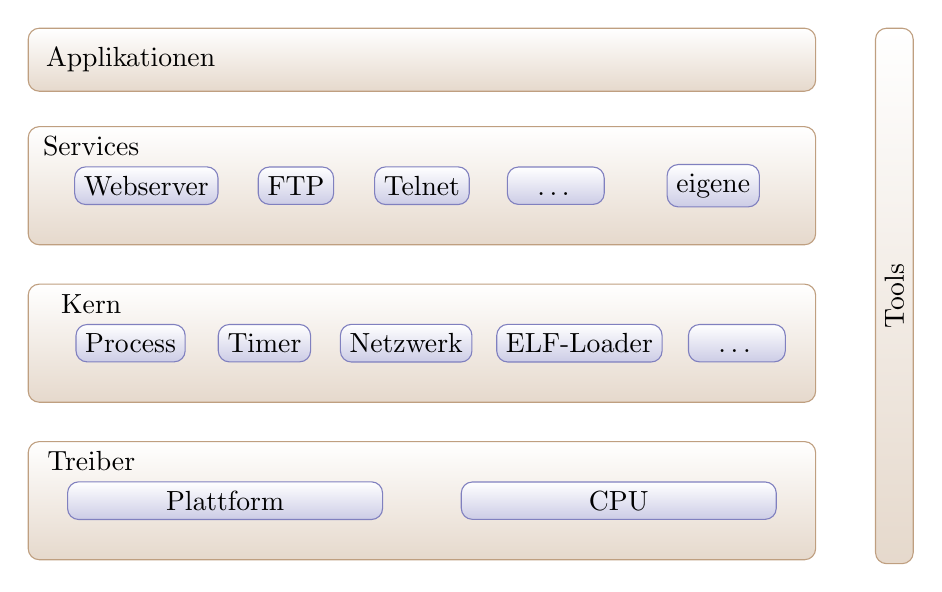
\begin{tikzpicture}
		\tikzstyle{subele}=[draw,
			rounded corners,
			top color=white,
			bottom color=blue!50!black!20,
			draw=blue!50!black!50,
			];
		\tikzstyle{ele}=[draw,
			rounded corners,
			top color=white,
			bottom color=orange!50!black!20,
			draw=orange!50!black!50,
			];

		\node [ele] at (0,5.6) [minimum width=10cm,minimum height=.8cm] {};
		\node at (-3.7,5.6) {Applikationen};

		\node [ele] at (0,4) [minimum width=10cm,minimum height=1.5cm] {};
		\node at (-4.2,4.5) {Services};
		\node [subele] at (-3.5,4) {Webserver};
		\node [subele] at (-1.6,4) {FTP};
		\node [subele] at (0,4) {Telnet};
		\node [subele] at (1.7,4) {\phantom{A}\dots\phantom{A}};
		\node [subele] at (3.7,4) {eigene};

		\node [ele] at (0,2) [minimum width=10cm,minimum height=1.5cm] {};
		\node at (-4.2,2.5) {Kern};
		\node [subele] at (-3.7,2) {Process};
		\node [subele] at (-2.0,2) {Timer};
		\node [subele] at (-.2,2) {Netzwerk};
		\node [subele] at (2,2) {ELF-Loader};
		\node [subele] at (4,2) {\phantom{A}\dots\phantom{A}};

		\node [ele] at (0,0) [minimum width=10cm,minimum height=1.5cm] {};
		\node at (-4.2,.5) {Treiber};
		\node [subele] at (-2.5,0) [minimum width=4cm] {Plattform};
		\node [subele] at (2.5,0) [minimum width=4cm] {CPU};

		\node [ele] at (6,2.6) [minimum width=6.8cm,rotate=90] {Tools};
	\end{tikzpicture}
	\captionbelow[Contiki-Schichten]{Contiki-Schichten nach \autocite{dreier10contikiblackfin}}
\label{fig:contiki_schichten}
\end{figure}

	Die Treiber kümmern sich dabei um die hardwarespezifischen Probleme.
	Die Kernmodule stellen die einzelnen Funktionalitäten, wie
	Multitasking oder fertige Timer, bereit.  Services nutzen diese
	Kernmodule, um \zB Netzwerkprotokolle bereitzustellen, die von
	Anwenderprogrammen genutzt werden können.

	\medskip

	Durch das angestrebte Einsatzgebiet (eingebettete, batteriebetriebene
	Systeme) ergeben sich zwei wichtige Anforderungen an das Betriebssystem:
	\begin{description}
	\item[Speicher]
		Da auf den Mikrocontrollern nur wenige \kilo\byte{} Speicher
		zur Verfügung stehen (\zB für den ATmega128RFA1
		\unita{16}{\kilo\byte}), muss das Betriebssystem mit
		möglichst wenig Speicher auskommen, damit für die eigentlichen
		Anwendungsprogrammen noch genug Speicher zur Verfügung steht.
	\item[Energie]
		Die Wartung der Hardware soll möglichst gering sein.
		Dazu muss ein Netzwerkknoten auch über Jahre mit nur einem
		Satz Batterien auskommen.
		Um dies gewährleisten zu können, muss das Betriebssystem
		die Stromsparmechanismen der Hardware unterstützen und optimal
		nutzen.
	\end{description}

	\medskip

	Der Aufbau dieses Dokuments gliedert sich daher wie folgt:

	In \autoref{sec:impl} wird das Konzept der Protothreads und die
	damit einhergehenden Möglichkeiten des Multitaskings sowie seine
	Beschränkungen als zentrales Programmiermodell in Contiki vorgestellt.
	In \autoref{sec:ns} wird speziell der Netzwerkstack von Contiki
	erklärt und analysiert.
	Abschließend wird in \autoref{sec:fazit} ein Fazit zum Contiki-OS gegeben.
